%%%%%%%%%%%%%%%%%%%%%%% file template.tex %%%%%%%%%%%%%%%%%%%%%%%%%
%
% This is a general template file for the LaTeX package SVJour
% for Springer journals.          Springer Heidelberg 2010/09/16
%
% Copy it to a new file with a new name and use it as the basis
% for your article. Delete % signs as needed.
%
% This template includes a few options for different layouts and
% content for various journals. Please consult a previous issue of
% your journal as needed.
%
%%%%%%%%%%%%%%%%%%%%%%%%%%%%%%%%%%%%%%%%%%%%%%%%%%%%%%%%%%%%%%%%%%%
%
% First comes an example EPS file -- just ignore it and
% proceed on the \documentclass line
% your LaTeX will extract the file if required
\begin{filecontents*}{example.eps}
%!PS-Adobe-3.0 EPSF-3.0
%%BoundingBox: 19 19 221 221
%%CreationDate: Mon Sep 29 1997
%%Creator: programmed by hand (JK)
%%EndComments
gsave
newpath
  20 20 moveto
  20 220 lineto
  220 220 lineto
  220 20 lineto
closepath
2 setlinewidth
gsave
  .4 setgray fill
grestore
stroke
grestore
\end{filecontents*}
%
\RequirePackage{fix-cm}
%
%\documentclass{svjour3}                     % onecolumn (standard format)
%\documentclass[smallcondensed]{svjour3}     % onecolumn (ditto)
%\documentclass[smallextended]{svjour3}       % onecolumn (second format)
\documentclass[twocolumn]{svjour3}          % twocolumn
%
% flush right qed marks, e.g. at end of proof
\smartqed

\usepackage[lofdepth,lotdepth]{subfig}
% \usepackage{graphicx}
%
\usepackage{mathptmx}      % use Times fonts if available on your TeX system
%
% insert here the call for the packages your document requires
\usepackage{amssymb}
\usepackage{amsmath}
\usepackage{amsfonts}
\usepackage{epstopdf}
\usepackage{mathrsfs} % para formato de letra
\usepackage{hyperref}
\usepackage{enumitem}
\usepackage{array}
\usepackage{tabularx}
\usepackage{supertabular}
\usepackage{fancyhdr}
\usepackage{multirow}
\usepackage{color}
\usepackage{makeidx}
\usepackage{xstring}
\usepackage{setspace}
\usepackage{epsfig}

\usepackage{pgf}
% \usepgfplotslibrary{external} 
% \tikzexternalize

%\usepackage{subfigure}
\usepackage{preview}
% Packages to write pseudo-algorithms %
\usepackage{algorithm}
\usepackage{algorithmic}

% Tikz
\usepackage{stanli}
\usepackage[ugly]{units}

%\usepackage{latexsym}
% etc.
%

% Matrix and vector nodes
\newcommand{\Matrix}[1]{
  \ensuremath{\mathbf{{#1}}}
}
\newcommand{\Vector}[1]{
  \ensuremath{\mathbf{{#1}}}
}

% Divergence
\newcommand{\Div}[1]{
  \ensuremath{\nabla \cdot {#1}}
}
% Gradient
\newcommand{\Grad}[1]{
  \ensuremath{\nabla{#1}}
}

% Partial derivative
\newcommand{\Deriv}[3][]{
  \ensuremath{\frac{\partial^{#1}{#2}}{ \partial {#3}^{#1} }}
}

% Integral
\newcommand{\Integral}[2]{
  \IfStrEqCase{#1}{
    {1}{\ensuremath{\int_{\Gamma}{#2}\ d\Gamma}}
    {2}{\ensuremath{\int_{\Sigma}{#2}\ d\Sigma}}
    {3}{\ensuremath{\int_{\Omega}{#2}\ d\Omega}}
  }
}

%
% Insert the name of "your journal" with
\journalname{Computational Particle Mechanics}
%
\begin{document}

\title{Suitability of the local-maximum entropy approximation under
  the Material Point Method framework for dynamic problems. \thanks{Funding: This
    study was funded by Agustín de Betancourt Foundation (grant number
    262390106114).}
}
% \subtitle{}

\titlerunning{Suitability of the LME approximation under
  the MPM framework for dynamic problems.}        % if too long for running head

\author{Miguel Molinos \and
  Pedro Navas \and
  Manuel Pastor \and
  Miguel Martín Stickle
}

%\authorrunning{Short form of author list} % if too long for running head

% \institute{Miguel Molinos \at
%   E.T.S de Ingenieros de Caminos, Canales y Puertos. \\
%   Universidad Politéctnica de Madrid, 28040 Madrid, Spain \\
%   \email{m.molinos@alumnos.upm.es}
%   % \emph{Present address:} of F. Author  %  if needed
%   \and
%   Pedro Navas 
%   \and
%   Manuel Pastor
%   \and
%   Miguel Martín Stickle
% }
% \institute{Miguel Molinos, Pedro Navas and Manuel Pastor \at E.T.S
%   de Ingenieros de Caminos, Canales y Puertos, Universidad Politéctnica de Madrid, 28040 Madrid, Spain, \; \email{m.molinos@outlook.es, pedro.navas@upm.es, manuel.pastor@upm.es}
% }


\date{Received: date / Accepted: date}
% The correct dates will be entered by the editor

\maketitle
\begin{abstract}
  This document is devoted to describe the suitability of the Local
  \textit{maximum-entropy} (LME) meshfree approximation technique under the framework of the
  Material Point Method for dynamic problems. 
  \keywords{LME \and MPM \and Dynamic problems}
  % \PACS{PACS code1 \and PACS code2 \and more}
  % \subclass{MSC code1 \and MSC code2 \and more}
\end{abstract}

\section{Introduction}
\label{intro}
Since the proposal of the Material Point Method (\textbf{MPM}) by Sulsky {\it
  et al.} (1994)\cite{Sulsky1994}, as a generalization of
a particle-in-cell method \cite{Harlow1956} and a fluid implicit
particle (FLIP) method \cite{Brackbill1986}, MPM has been used to
simulate dynamic problems. However, in the simulations made with the
originalMPM, there are numerical noises \cite{Tran2019e} when it is faced to solve
classic dynamic benchmarks like the one proposed by Dyka \& Ingel
(1995)\cite{Dyka1995}. 

The aim of this paper is to mitigate this spurious oscillations by the
employ of the maximum-entropy (or local \textit{max-ent}) shape
function under the MPM framework. First introduced by
\cite{Arroyo2006}, it belongs to the class of convex 
approximation schemes and provides a seamless transition between
finite elements (\textbf{FE}) and mesh-free interpolations. The
approximation scheme is based on a compromise between minimizing the
width of the shape function support and maximizing the information
entropy of the approximation. The local \textit{max-ent} approximation
may be regarded as a regularization, or \textit{thermalization}, of
Delaunay triangulation which effectively resolves the degenerate cases
resulting from the lack of uniqueness of the triangulation. Local
\textit{max-ent} basis functions possess many desirable properties for
meshfree algorithms. First of all, they are entirely defined by the
nodal set and the domain of analysis. They are also non-negative, satisfy the partition of unity
property, and provide an exact approximation for affine functions \cite{Arroyo2006}.

This approximation scheme has been proof to have a good performance
under the dynamic regime by other researchers like Navas {\it et al.}
(2018)\cite{Navas2018a} and Li {\it et al.} (2012)\cite{Li2012} for
Optimal Transportation Meshfree (\textbf{OTM}) method.

a comparison between both methods employing \textit{max-ent}  shape
function is performed in this paper

as well a parametric study for the $\gamma$ parameter

finally, conclusions and future research topics are exposed

\section{Overview of the MPM}
\label{sec:mpm-overview}
In this section, we provide an overview of the standard explicit MPM
algorithm as presented by \cite{Sulsky1994}. The method has three main
steps: a variational recovery process to project particle data to the
nodes of the grid, a Eulerian step where balance of momentum is
compute by solving internal and external forces in the nodes, and
finally the advection of the Lagrangian particles. We will first give
a introduction to the governing equations and then follow by an
algorithmic description of the process.

\subsection{Derivation of the MPM}
\label{sec:derivation-mpm}
In the MPM approach a continuum is considered. The continuum behaviour
can be described by a set of governing equations which are the balance
of momentum equation ($\rho \vect{a} = \Div{\tens{\sigma}} + \rho
\vect{b}$), the compatibility equation ($\dot{\tens{\varepsilon}} =
\Grad{\vect{v}}$), the constitutive equation ($\dot{\tens{\sigma}} =
\tens{D} \colon \dot{\tens{\varepsilon}}$), and the balance of mass equation
($\frac{D \rho}{D t} = \dot{\rho} + \rho \Grad{\vect{v}}$). The balance of momentum can be
formulated in weak form by introducing an arbitrary test function $\vec{\psi}$, yielding
\begin{equation}
  \label{eq:BalanceMomentum_wf}
  \Integral{3}{\rho\ \Deriv{\vec{v}}{t}\ \vec{\psi}} = -
  \Integral{3}{\tens{\sigma} \colon \Grad{\vec{\psi}}} +
  \Integral{2}{\vec{t}\ \vec{\psi}} + \Integral{3}{
  \rho\ \vec{b}\ \vec{\psi}}.
\end{equation}\\

In order to arrive to a finite set of equations, the continuum domain
$\Omega$ is discretized with a finite sum of particles (material points), each one 
represent a part of the domain $\Omega_p$ with $p = 1,2\ldots ,N_p$
where $N_p$ is the number of particles. The index $p$ is
used for the particles, while the index $I$ is reserved in this
notation for denoting grid nodes. The material point $\vec{x}_p$ is
defined at the centroid of $\Omega_p$. Further, a computational grid
is formed of a finite set of grid points with coordinates $\vec{x}_I\
, I = 1,2\ldots ,N_n$, where $N_n$ is the number of grid nodes. Each material point is assigned with initial values of position,
velocity, mass, volume and stress denoted by $\vec{x}_p$,  $\vec{v}_p$, $m_p$,  $V_p$ and $\tens{\sigma}_p$. The problem is then integrated using a discrete number of time
steps $k = 1\ldots ,Nt$, where $k$ is the current time step and $N_t$
is the total number of time steps.  So employing the definition of the
material integral, individual terms of \eqref{eq:BalanceMomentum_wf}
are solved as follows. 
\begin{itemize}
\item Acceleration forces :
\begin{equation}
    \label{eq:particle_acceleration_forces}
    \Integral{3}{\rho\ \vec{a}\ \vec{\psi}} =& \sum^{N_p}_{p}
   \dot{\vec{v}}_{p}\ \vec{\psi}_{p}\ m_p.
  \end{equation}\\
\item Internal forces :
  \begin{equation}
    \label{eq:particle_internal_forces}
    \Integral{3}{\tens{\sigma}\ \colon \Grad{\vec{\psi}}} = \sum^{N_p}_{p}
   \tens{\sigma}_{p}\ \Grad{\tens{\psi}_{p}}\ V_p.
  \end{equation}\\
\item Body forces :
\begin{equation}
  \label{eq:particle_body_forces}
  \Integral{3}{\rho\ \vec{b}\ \vec{\psi} } = \sum^{N_p}_{p}
  \vec{b}_{p}\ \vec{\psi}_{p}\ m_p.
\end{equation}\\
\item Loads :
\begin{equation}
  \begin{aligned}
    \label{eq:particle_load_forces}
    \Integral{2}{\vec{t}\ \vec{\psi}} = \Integral{2}{\rho\
      \vec{t}^s\ \vec{\psi}} = \sum^{N_p}_{p} \vec{t}^s_{p}\ \vec{\psi}_{p}\ h^{-1}\ m_p ,
  \end{aligned} 
\end{equation}
\end{itemize}
where $h$ is the thickness of the continuum in a 2D case. Introducing \eqref{eq:particle_acceleration_forces},
\eqref{eq:particle_internal_forces}, \eqref{eq:particle_body_forces},
and \eqref{eq:particle_load_forces} in \eqref{eq:BalanceMomentum_wf}
we reach to the particle balance of forces of the continuum,
\begin{equation}
  \label{eq:particle_balance_forces2}
  \sum^{N_p}_{p}\vec{\psi}_{p}\ m_p\ \dot{\vec{v}}_{p} = \sum^{N_p}_{p}
  \vec{\psi}_{p}\ m_p\ \vec{b}_{p} + \sum^{N_p}_{p}
  \vec{\psi}_{p}\ m_p\ h^{-1}\ \bar{\vec{t}}^s_{p} -
  \sum^{N_p}_{p} \Grad{\vec{\psi}_{p}}\ \frac{m_p}{\rho_p}\
  \tens{\sigma}_{p}.
\end{equation}\\

Approximating the virtual displacement of the particle $\vec{\psi}_{p}$
using a suitable approximation scheme we get \eqref{eq:VirtualDisplacementParticle}.
\begin{equation}
  \label{eq:VirtualDisplacementParticle}
  \vec{\psi}_{p} = N_{Ip}\cdot \vect{1} = N_{Ip},
\end{equation}
where $N_{Ip} = N_I(\vec{x}_p)$ it is the nodal value of the shape
function evaluated in the material point coordinates denoted by $\vec{x}_p$. Substituting \eqref{eq:VirtualDisplacementParticle} in
\eqref{eq:particle_balance_forces2} we get :
\begin{equation}
  \label{eq:particle_balance_forces3}
  \dot{\vec{p}}_{I}= \tens{m}_{IJ}\dot{\vec{v}}_{J} = \vec{f}_{I}^{int} + \vec{f}_{I}^{ext},
\end{equation}
where $\dot{\vec{p}}_{I}$ is the rate of momentum at grid node $I$, the nodal mass matrix $\tens{m}_{IJ}$ is,
\begin{equation}
  \label{eq:particle_nod_mass}
  \tens{m}_{IJ} =
  \sum^{Np}_{p} N_{Ip} m_p N_{Jp},
\end{equation}
and internal and external forces are computed as follows,
\begin{equation}
  \label{eq:nodal_internal_forces}
  \vec{f}_{I}^{int} = - \sum^{N_p}_{p} \Grad{N_{Ip}}
  \tens{\sigma}_{p} \frac{m_p}{\rho_p}
\end{equation}
\begin{equation}
  \label{eq:nodal_external_forces}
  \vec{f}_{I}^{ext} = \sum^{N_p}_{p} N_{Ip} m_p \vec{b}_{p} + \sum^{N_p}_{p}
  N_{Ip} m_p h^{-1} \vec{t}^s_{p}
\end{equation}
where $\tens{\sigma}_{p} = \tens{\sigma}_{p}(\tens{\varepsilon}_{p})$
is the particle $p$ stress field, which can be integrated employing
the suitable constitutive model. The strain tensor is updated employing the rate of stress tensor $\dot{ \tens{\varepsilon}}_{p}$ used to update the
strain tensor is as follows \eqref{eq:IncrStrainPoint}.
\begin{equation}
  \label{eq:IncrStrainPoint}
  \dot{\tens{\varepsilon}_{p}} = \frac{\Delta
    \tens{\varepsilon}_{p}}{\Delta t} =
  \frac{1}{2}\left[\Grad{N_{Ip}}\ \vec{v}_{I} + \Grad{N_{Ip}}^T\
    \vec{v}_{I}\right].
\end{equation}
Later, imposing $\frac{D \rho}{D t} = 0$, we ensures the mass
conservation and update the density field.
\begin{equation}
  \label{eq:MassConservation}
\dot{\rho} = - \rho\ \mathit{tra} \left( \dot{\tens{\varepsilon}} \right)
\end{equation}

To improve the computational efficiency and stability, the nodal mass matrix
\eqref{eq:particle_nod_mass} can be substituted by the lumped mass
matrix $\tens{m}_I$. Therefore the nodal balance of momentum equation \eqref{eq:particle_balance_forces3} can be simplified to
\begin{equation}
  \label{eq:SimplyNodalMomentum}
  \dot{\vec{p}}_{I} = \tens{m}_I\ \vec{a}_{I} = \vec{f}_{I}^{int} + \vec{f}_{I}^{ext}.
\end{equation}
To solve the equation \eqref{eq:SimplyNodalMomentum}, a second order
temporal integration scheme is required. The next step is to advect
the particles solving,
\begin{equation}
  \label{eq:Updated_Lagrangian}
  \dot{\vec{v}}_p = \sum^{N_n}_{I}\vec{a}_{I}\ N_{Ip},\quad and\quad \dot{\vec{x}}_{p} = \sum^{N_n}_{I}\vec{v}_{I}\ N_{Ip}  
\end{equation}
To solve this equations, the forward Euler algorithm is the common
choose for this in the MPM literature. In next lines, a complete
description of the standard MPM algorithm will be described.

\section{Explicit predictor-corrector scheme for MPM.}
\label{sec:epc-algor-mpm}

To solve equations \eqref{eq:SimplyNodalMomentum} and
\eqref{eq:Updated_Lagrangian}, a time integration scheme is
required. It has been described in detail by many researchers
\cite{Sulsky1994}, \cite{Bardenhagen2002}, \cite{thesis_Andersen_2009} and summarized
in Figure \ref{fig:MPM_algorithm}. Other authors have proposed many
others time integration alternatives like
\cite{Guilkey2003}, \cite{Tran2019e}, \cite{Charlton2017}. In the first publication on
the MPM \cite{Sulsky1994}, the nodal acceleration in employed to
update the particles as
\begin{equation}
  \label{eq:Sulsky-1994-UL-v-x}
  \vect{v}_p^{k+1} = \vect{v}_p^{k} + \Delta t\
  \sum^{N_n}_{I}N_{Ip}^{k}\ \vec{a}_{I}^{k},\quad and\quad
  \vect{x}_p^{k+1} = \vect{x}_p^{k} + \Delta t\ \sum^{N_n}_{I}N_{Ip}^{k}\ \vec{v}_{I}^{k}.
\end{equation}

However, in Andersen (2009)\cite{thesis_Andersen_2009} this
algorithm has been shown to be numerically unstable due to that
$\vect{f}_I^{int,k}$ can be finite for an infinitesimal nodal mass
$\tens{m}$. This can lead to numerical issues when nodal acceleration
is obtained for evaluating \eqref{eq:Sulsky-1994-UL-v-x}. Hence, a
corrected version of this algorithm in shown in Zhang {\it et al.}
(2016)\cite{Zhang_book_2016}
\begin{equation}
  \label{eq:Zhang-2016-UL-v-x}
  \vect{v}_p^{k+1} = \vect{v}_p^{k} + \Delta t\
  \sum^{N_n}_{I}\frac{N_{Ip}^{k}\ \vec{f}_{I}^{k}}{\tens{m}_I},\quad and\quad
  \vect{x}_p^{k+1} = \vect{x}_p^{k} + \Delta t\ \sum^{N_n}_{I} \frac{N_{Ip}^{k}\ \vec{p}_{I}^{k}}{\tens{m}_I}.  
\end{equation}

Later Tran \& Solowski (2019)\cite{Tran2019e} presented a
generalized-$\alpha$ scheme for the MPM inspired in the explicit time
integration algorithm proposed by Chung \& Hulbert
(1993)\cite{Geranlized_alpha_1993}, but with the particularity that
the acceleration is evaluated both in the beginning and the end of the
time step.
\begin{align}
  \label{eq:Tran-2019-GA-v}
  & \vect{v}_p^{k+1} = \vect{v}_p^{k} + \Delta t\
    \sum^{N_n}_{I} N_{Ip}^{k}\ \left[(1 - \gamma)\ \vect{a}_I^{k} +
    \gamma\ \vect{a}_I^{k+1} \right]\\
  \label{eq:Tran-2019-GA-x}
  & \vect{x}_p^{k+1} = \vect{x}_p^{k} + \Delta t\
    \sum^{N_n}_{I}N_{Ip}^{k}\ \vec{v}_{I}^{k} + \Delta t^2
    \sum^{N_n}_{I}N_{Ip}^{k} \left[ (\frac{1}{2} - \beta)\
    \vec{a}_{I}^{k} + \beta\ \vec{a}_{I}^{k+1} \right]
\end{align}
and
\begin{equation}
  \label{eq:Tran-2019-GA-a}
   \vect{a}_p^{k+1} = \sum^{N_n}_{I}N_{Ip}^{k}\ \vec{a}_{I}^{k+1}.
\end{equation}

This scheme has prof to damps out the higher frequency noises
\cite{Tran2019e}. But it can present the same numerical instabilities
as in \eqref{eq:Sulsky-1994-UL-v-x} when nodal masses become infinitesimal.
Here we propose a explicit predictor-corrector scheme for MPM based on the Newmark a-form with
$\gamma = 0.5$ and $\beta = 0$ which is the central difference
explicit. This method is devoted to solve a system of equations of type
\begin{equation*}
  \Matrix{M}_{IJ}\ddot{\Vector{d}}_{J} + \Matrix{C}_{IJ}\dot{\Vector{d}}_{J} +
  \Matrix{K}_{IJ}\Vector{d}_{J} = \Vector{F}_{I}
\end{equation*}
Nevertheless it can be applied for an isolated mass, therefore it is
possible to apply this methods successfully in the MPM framework as
was proved by \cite{Tran2019e}. Taking the predictor
definition from the classic literature \cite{Hughes2000} and
calculating particles velocity and acceleration as described in 
\cite{Zhang_book_2016}, we get the following expression for the
\textbf{predictor} stage for both velocity and displacement.
\begin{align}
  \label{eq:Predictor-displacement}
  &\vec{x}_p^{n+1} = \vec{x}_p^n + \Delta t\ \underbrace{\sum^{N_n}_{I}\frac{\vec{p}_{I}^{k}\ N_{Ip}^k}{\tens{m}_I^k}}_{\vec{v}_p^{n}} + \frac{1}{2}\Delta t^2\ \underbrace{\sum^{N_n}_{I}\frac{\vec{f}_{I}^{k}\ N_{Ip}^k}{\tens{m}_I^k}}_{\vec{a}_p^{n}}\\
  \label{eq:Predictor-velocity}
  &\vec{v}_p^{n+1} = \vec{v}_p^n + (1 - \gamma)\ \Delta t\ \underbrace{\sum^{N_n}_{I}\frac{\vec{f}_{I}^{k}\ N_{Ip}^k}{\tens{m}_I^k}}_{\vec{a}_p^{n}}        
\end{align}

Consequently, the \textbf{corrector} stage for the particles velocity is in the
following way
\begin{equation*}
  \vec{v}_{p}^{k+1} = \vec{v}_{p}^{k+1} +
  \gamma\ \Delta t\ \underbrace{\sum^{N_n}_{I}\frac{\vec{f}_{I}^{k+1}\ N_{Ip}^{k+1}}{\tens{m}_I^{k+1}}}_{\vec{a}_p^{n+1}}  
\end{equation*}

Notice that the predictor of the particle displacement is
computed using information only from the predictor of the
previous step. However, velocities are computed using half information
of the past corrector and half of the past predictor. Therefore here we share
similarities with the \textbf{leapfrog integration} which updates the
position at full time step, but updates the velocity at half time
steps. Due to its simplicity allows be implemented with minor modifications
over a standard forward Euler. It is summarized in shape of
pseudo-algorithm \ref{alg:PCE-algorithm}.

\begin{algorithm}
\floatname{algorithm}{Algorithm}
\renewcommand{\thealgorithm}{}
\caption{Explicit scheme : Newmark central difference}
\label{alg:Second_step_MPM_2STG}
\begin{algorithmic}[1]
  %%%%%%%%%%%%%%%%%%%%%%%%%%%%%%%%%%%%%%%%%%%%%%%%%%%%%%%%%%%%%%%%%%%%%%%%%%%%%%%%%%%%%% º
  \STATE \textbf{Explicit Newmark Predictor} ($\gamma = 0.5$) :
  \begin{align*}
    &\vec{x}_p^{n+1} = \vec{x}_p^n + \Delta t\ \sum^{N_n}_{I}\frac{\vec{p}_{I}^{k}\ N_{Ip}^k}{\tens{m}_I^k} + \frac{1}{2}\Delta t^2\ \sum^{N_n}_{I}\frac{\vec{f}_{I}^{k}\ N_{Ip}^k}{\tens{m}_I^k}\\
    &\vec{v}_p^{n+1} = \vec{v}_p^n + (1 - \gamma)\  \sum^{N_n}_{I}\frac{\vec{f}_{I}^{k}\ N_{Ip}^k}{\tens{m}_I^k}\Delta t        
  \end{align*}
  %%%%%%%%%%%%%%%%%%%%%%%%%%%%%%%%%%%%%%%%%%%%%%%%%%%%%%%%%%%%%%%%%%%%%%%%%%%%%%%%%%%%%% 
  \STATE \textbf{Discard the previous nodal values}.
  %%%%%%%%%%%%%%%%%%%%%%%%%%%%%%%%%%%%%%%%%%%%%%%%%%%%%%%%%%%%%%%%%%%%%%%%%%%%%%%%%%%%%% 
  \STATE \textbf{Transference of particles kinetics information to the
    mesh}:\\
  Calculate the lumped mass matrix \eqref{eq:Lumped-mass-matrix},
  and later the nodal momentum \eqref{eq:Nodal-momentum} of the
  corrected values.
  \begin{equation*}
    \tens{m}_{I} = \sum_{p}^{N_p} m_p\ N_{Ip}^{k+1},\quad
    \vec{p}_{I}^{k+1} = \sum_{p}^{N_p} m_p\ \vec{v}_{p}^{k+1}\ N_{Ip}^{k+1},\quad
    \vec{v}_{I}^{k+1} = \frac{\vec{p}_{I}^{k+1}}{\tens{m}_I}.
  \end{equation*}
  %%%%%%%%%%%%%%%%%%%%%%%%%%%%%%%%%%%%%%%%%%%%%%%%%%%%%%%%%%%%%%%%%%%%%%%%%%%%%%%%%%%%%% 
  \STATE \textbf{Impose essential boundary conditions over the nodal
    values}:\\
  At the fixed boundary, set $\vec{p}_{I}^{k+1} = 0$.
  %%%%%%%%%%%%%%%%%%%%%%%%%%%%%%%%%%%%%%%%%%%%%%%%%%%%%%%%%%%%%%%%%%%%%%%%%%%%%%%%%%%%%% 
  \STATE \textbf{Deformation tensor increment calculation}.
  \begin{align*}
    &\dot{\tens{\varepsilon}_{p}}^{k+1} = \frac{1}{2}\ \sum_{I}^{N_n}
    \Grad{N_{Ip}^{k+1}}\vec{v}_{I}^{k+1} +
      (\Grad{N_{Ip}^{k+1}}\vec{v}_{I}^{k+1})^T \\
    &\Delta \tens{\varepsilon}_{p}^{k+1} = \Delta t\ \dot{\tens{\varepsilon}_{p}}^{k+1}
  \end{align*}
  %%%%%%%%%%%%%%%%%%%%%%%%%%%%%%%%%%%%%%%%%%%%%%%%%%%%%%%%%%%%%%%%%%%%%%%%%%%%%%%%%%%%%% 
  \STATE \textbf{Update the density field}:\\
  Imposing the mass conservation in the total derivative expression of
  the density field we reach to a suitable way of update it.
  \begin{equation*}
    \rho_p^{k+1} = \frac{\rho_p^k}{1 + \mathit{tra}\left[\Delta\tens{\varepsilon}_{p}^{k+1}\right]}.
  \end{equation*}
  %%%%%%%%%%%%%%%%%%%%%%%%%%%%%%%%%%%%%%%%%%%%%%%%%%%%%%%%%%%%%%%%%%%%%%%%%%%%%%%%%%%%%% 
  \STATE \textbf{Balance of forces calculation}:\\
  Calculate the grid nodal internal forces $\vec{f}_{I}^{int,k+1}$, external
  forces $\vec{f}_{I}^{ext,k+1}$, and the total grid nodal force $\vec{f}_{I}^{k+1} =
  \vec{f}_{I}^{int,k+1} + \vec{f}_{I}^{ext,k+1}$ evaluating
  \eqref{eq:nodal_internal_forces} and
  \eqref{eq:nodal_external_forces} in the time step $k+1$. In the
  grid node $I$ is fixed in one of the spatial dimensions, set it to
  zero to make the grid nodal acceleration zero in that direction.\\
  %%%%%%%%%%%%%%%%%%%%%%%%%%%%%%%%%%%%%%%%%%%%%%%%%%%%%%%%%%%%%%%%%%%%%%%%%%%%%%%%%%%%%% 
  \STATE \textbf{Integrate the grid nodal momentum equation :}\\
  Following the definition \eqref{eq:particle_balance_forces3}
  calculate the nodal momentum $\vec{p}_{I}$ in $k+1$. 
  \begin{equation*}
    \vec{p}_{I}^{k+1} = \vec{p}_{I}^{k} + \vec{f}_{I}^{k+1}\Delta t
  \end{equation*}
  %%%%%%%%%%%%%%%%%%%%%%%%%%%%%%%%%%%%%%%%%%%%%%%%%%%%%%%%%%%%%%%%%%%%%%%%%%%%%%%%%%%%%% 
  \STATE \textbf{Explicit Newmark Predictor}:
  \begin{equation*}
    \vec{v}_{p}^{k+1} = \vec{v}_{p}^{k+1} +
    \gamma \sum^{N_n}_{I}\frac{\vec{f}_{I}^{k+1}\ N_{Ip}^{k+1}}{\tens{m}_I^{k+1}}\Delta t  
  \end{equation*}
  %%%%%%%%%%%%%%%%%%%%%%%%%%%%%%%%%%%%%%%%%%%%%%%%%%%%%%%%%%%%%%%%%%%%%%%%%%%%%%%%%%%%%% 
\end{algorithmic}
\end{algorithm} 

\begin{figure}\sidecaption
  \centering
  \resizebox{0.6\hsize}{!}{
    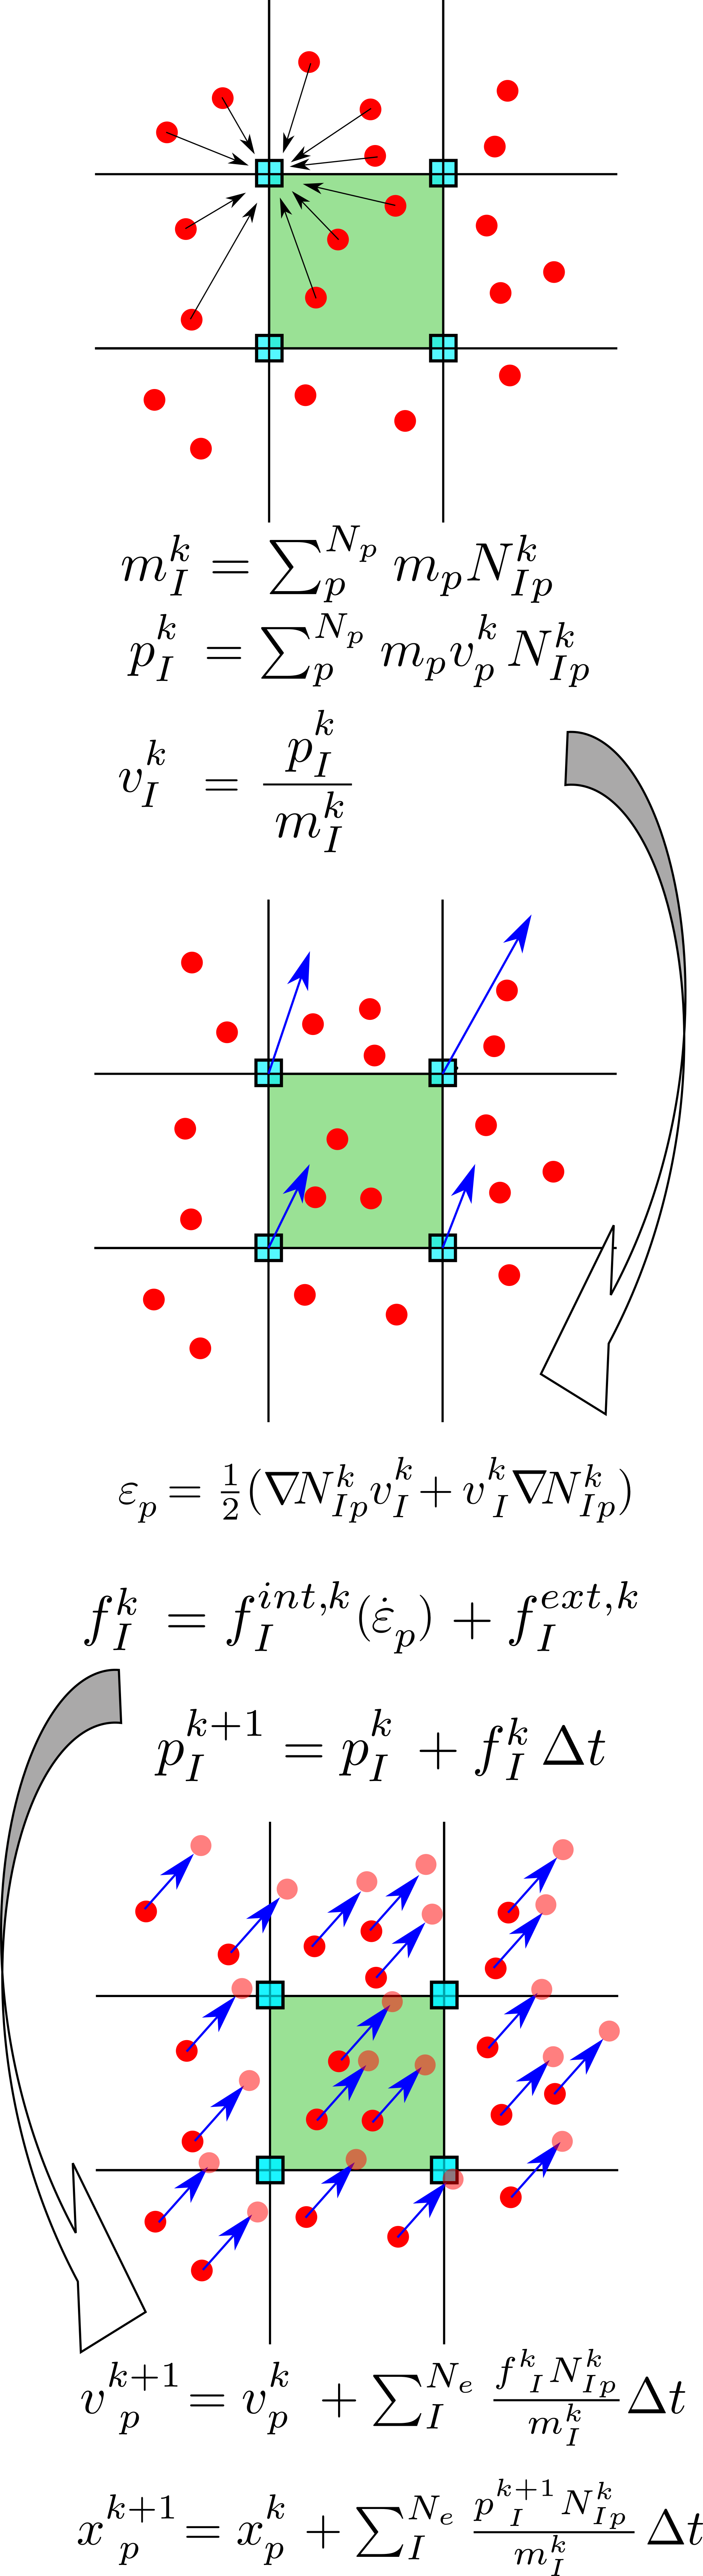
\includegraphics[width=\textwidth]{./Figures/MPM_scheme}
  }
  \caption{MPM standard algorithm.}
  \label{alg:PCE-algorithm}
\end{figure}

\section{Local max-ent approximants}
\label{sec:local-max-ent}

The previous lines describe the main algorithm without defining an
interpolation technique. A direct consequence of this, is that it is
possible to adopt a width range of shape functions and interpolation techniques. The MPM has been
successfully applied to a wide range of problems due to its ability to
deal with large strain problems without mesh distorsion issues inherent to
mesh based methods like FE. However, in the simulations made with the
original MPM, there are numerical noises when particles crossing
the cell boundaries. These numerical inaccuracies give rise to the
development of other interpolation techniques. Some of this
alternatives techniques are the generalized interpolation material
point method (GIMP) Bardenhagen \& Kober (2004)\cite{Bardenhagen2004},
the dual domain material point method (DDMP) Zhang {\it et al.}
(2011)\cite{Zhang2011a}, the B-Spline MPM Tran {\it et al.}
(2019)\cite{Tran2019a}, the Conservative Taylor Least
Squares reconstruction Wobbes {\it et al.}
(2018)\cite{E_Wobbes_2018} and more recently the local
maximum-entropy (or local \textit{max-ent}) shape function first
introduced by Arroyo \& Ortiz (2006)\cite{Arroyo2006} has been tested
under the MPM framework by Wobbes {\it et al.}
(2020)\cite{Wobbes2020} where they prof that simulations performed with the maxent basis functions
show considerably more accurate stress approximations for
MPM. Although, in \cite{Wobbes2020} authors does not deep in $\beta$
parameter benefits

The maximum-entropy estimate is defined as the type of statistical
inference, which is the least biased possible on the given information
\cite{Jaynes1957}. The basic idea of the shape functions based on such an estimate is to interpret the shape function $N_I(\vec{x})$ as the probability of $\vec{x}$ to obtain the value $\vec{x}_I$,  $I=1, \dots, n$. Here $n$ is the number of nodes in the domain. Taking Shannon's entropy as the starting point:
\begin{equation}
  \label{eq:Shannon-entropy}
  H(p_1(\vec{x}),...,p_n(\vec{x})) = -\sum^{N_n}_{I=1}{p_I(\vec{x})\log p_I }
\end{equation}
where $p_I(\vec{x})$ is the probability, equivalent to the mentioned
shape function $N_I(\vec{x})$,  satisfying both the zeroth and
first-order consistency. The least-biased approximation scheme is given by
\begin{eqnarray}
  \text{(ME)} \hspace{0.2cm} \text{Maximize} \hspace{0.1cm}H(p) &=&  -\sum_{I}^{N_n}{p_I(\vec{x})\log p_I } \nonumber \\
  \text{subject to} \hspace{0.5cm} p_I &\ge& 0, \hspace{0.5cm} \text{I=1, ..., n} \nonumber \\
  \sum_{I=1}^{N_n}{p_I} &=& 1 \nonumber \\
  \sum_{I=1}^{N_n}{p_I \vec{x}_I} &=& \vec{x} \nonumber 
\end{eqnarray}
The local max-ent approximation schemes (LME) as a Pareto set,
defined by \cite{Arroyo2006} is as follows 
\begin{eqnarray}
  \text{(LME)}_{\beta} \hspace{0.5cm} \text{For fixed} \hspace{0.2cm} \vec{x} \hspace{0.2cm} \text{minimise}  \nonumber \\
  \hspace{0.5cm}f_{\beta}(\vec{x}, p) &=& \beta H(\vec{x},p) - H(p)  \nonumber  \\
  \text{subject to} \hspace{0.5cm} p_I &\ge& 0, \hspace{0.2cm} \text{I=1, ..., n}  \nonumber \\
  \sum_{I=1}^{N_n}{p_I} &=& 1  \nonumber \\
  \sum_{I=1}^{N_n}{p_I \, \vec{x}_I} &=& \vec{x}    \nonumber 
\end{eqnarray}
for $\beta \in (0,\infty)$ is Pareto optimal. The unique solution of
the local max-ent problem (LME)$_\beta$ is: 
\begin{equation}
  \label{eq:LME-p}
p(\vec{x})=\frac{\exp\left[ -\beta \; |\vec{x}-\vec{x}_I|^2 +  \vec{\lambda}  \;  (\vec{x}-\vec{x}_I)         \right] } {Z(\vec{x},\vec{\lambda}^*(\vec{x}))}
\end{equation}
where
\begin{equation}
  \label{eq:LME-Z}
Z(\vec{x}, {\vec{\lambda}}) = \sum_{I=1}^{N_n}{ \exp \left[ -\beta \, | \vec{x}-\vec{x}_I|^2 + \vec{\lambda}  \,  (\vec{x}-\vec{x}_I)  \right]}
\end{equation}
being $\vec{\lambda}^*(\vec{x})$ the unique minimiser  for $\log Z(\vec{x}, \vec{\lambda})$

In order to obtain the first derivatives of the shape function, it is  also necessary to compute~$\nabla p^*_I$ 
\begin{equation}
  \label{eq:LME-grad-p}
\nabla p^*_I=p^*_I  \, \left(\nabla f^*_I-\sum_J^{N_n} p^*_J \, \nabla f^*_J\right)
\end{equation}
where
\begin{equation}
  \label{eq:LME-f}
f^*_I(\vec{x},  \vec{\lambda},\beta)=-\beta \, |\vec{x}-\vec{x}_I|^2 + \vec{\lambda}   \,  (\vec{x}-\vec{x}_I)
\end{equation}
Employing the chain rule, rearranging and considering $\beta$ as a constant, Arroyo and Ortiz~\cite{Arroyo2006} obtained the following expression:
\begin{eqnarray}
\nabla p^*_I &=& -p^*_I \,  (\tens{J}^*)^{-1} \,  (\vec{x} - \vec{x}_I) \label{eq26} 
\end{eqnarray}
%&&\mbox{
where \tens{J} is the Hessian matrix, defined by:
%} \nonumber \\&& \nonumber \\
\begin{eqnarray}
\tens{J}(\vec{x},  \vec{\lambda},\beta) &=& \frac{\partial \vec{r}}{\partial  \vec{\lambda}} \label{eq27} \\ 
%&& \nonumber \\
\vec{r}(\vec{x},\vec{\lambda},\beta) &\equiv& \partial_{\vec{\lambda}}{\log{ Z( \vec{x},\vec{\lambda}})} 
%\nonumber \\ &=&
  =\sum_I^{N_n} p_I(\vec{x},\vec{\lambda},\beta) \, (\vec{x} - \vec{x}_I) \label{eq28} 
\end{eqnarray}
Note that, the objective of the above procedure is to find the $\vec{\lambda}$ which minimises  $\log Z(\vec{x}, \vec{\lambda})$. 
The traditional way to obtain such a minimiser  is using Eq.~(\ref{eq27}) to calculate small increments of $\partial\vec{\lambda}$ in a Newton-Raphson approach. 

Similar to alternative non-polynomial meshfree basis functions, the LME approximation scheme requires more than $d+1$ nodes to determine the values of the shape functions as well as their derivatives at any point in the convex hull of the nodal set, where $d$ is the dimension of the problem. Due to the FE-compatibility, the LME shape function is degenerated to linear finite element shape function if $d+1$ neighbouring nodes are chosen as the support. The support size of LME shape functions may be controlled by adjusting a dimensionless parameter, $\gamma=\beta h^2$ (e.g. two dimensional example shown in Fig. \ref{fig:LME_MPM})\cite{Arroyo2006}.
Since  $p_I$  is defined in  the entire domain, in practice,  the function $\exp(-\beta \vec{r} )$ truncated  by  a given tolerance, 10$^{-6}$, for example,  would ensure a reasonable range of neighbours, see \cite{Arroyo2006} for details. This  tolerance defines the limit values of the influence radius and   is used thereafter to find the neighbour nodes of a given integration point.

\begin{figure}
  \centering
  %%%%%%%%%%%%%%%%%%%%%%%%%%%%%%%%%%%%%%%%%%%%%% 
  \subfloat{
    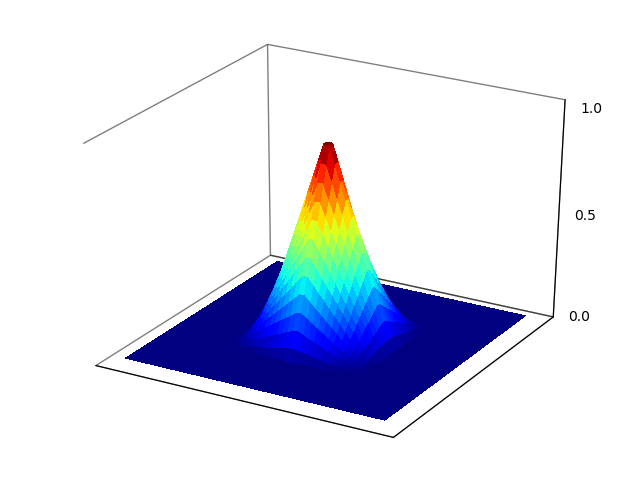
\includegraphics[width=0.35\columnwidth]{Figures/MPM_Shape_Fun.png}
    % \resizebox{0.3\columnwidth}{!}{%
    % \input{Figures/MPM_Shape_Fun.png}
    % }
    \label{fig:MPM_Shape_Fun}
  }
  \subfloat{
    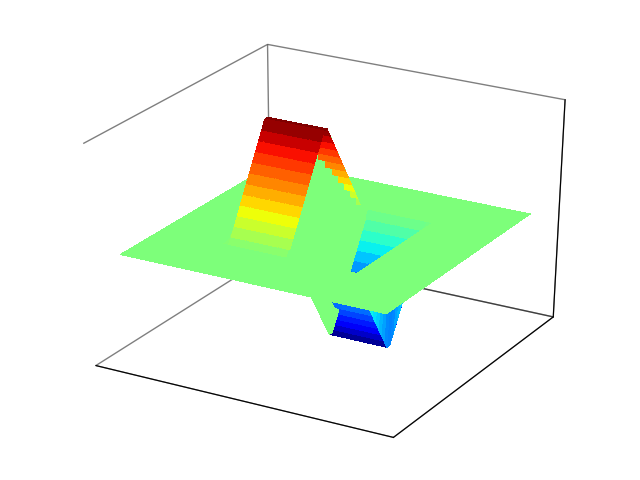
\includegraphics[width=0.35\columnwidth]{Figures/MPM_Shape_Fun_dx.png}
    % \resizebox{0.54\columnwidth}{!}{%
    % \input{Figures/MPM_Shape_Fun_dx.png}
    % }
    \label{fig:MPM_Shape_Fun_dx}
  }
  \subfloat{
    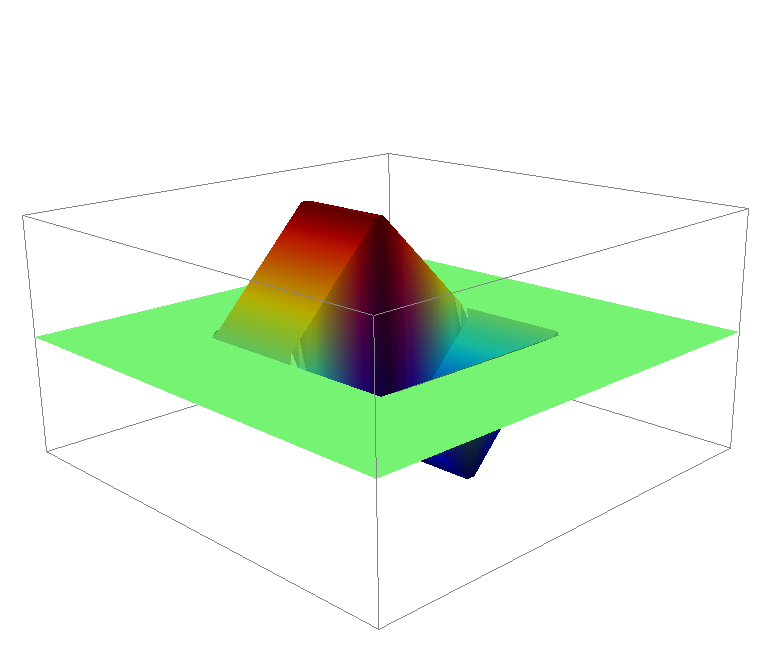
\includegraphics[width=0.35\columnwidth]{Figures/MPM_Shape_Fun_dy.png}
    % \resizebox{0.54\columnwidth}{!}{%
    % \input{Figures/MPM_Shape_Fun_dy.pgf}
    % }
    \label{fig:MPM_Shape_Fun_dy}
  }
  %%%%%%%%%%%%%%%%%%%%%%%%%%%%%%%%%%%%%%%%%%%%%% 
  \qquad
  %%%%%%%%%%%%%%%%%%%%%%%%%%%%%%%%%%%%%%%%%%%%%% 
  \subfloat{
    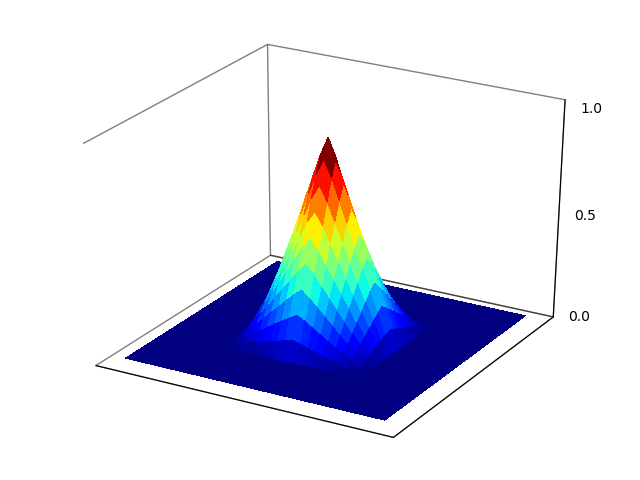
\includegraphics[width=0.35\columnwidth]{Figures/LME_17.3_Shape_Fun.png}
    % \resizebox{0.3\columnwidth}{!}{%
    % \input{Figures/LME_17.3_Shape_Fun.png}
    % }
    \label{fig:LME_17.3_Shape_Fun}
  }
  \subfloat{
    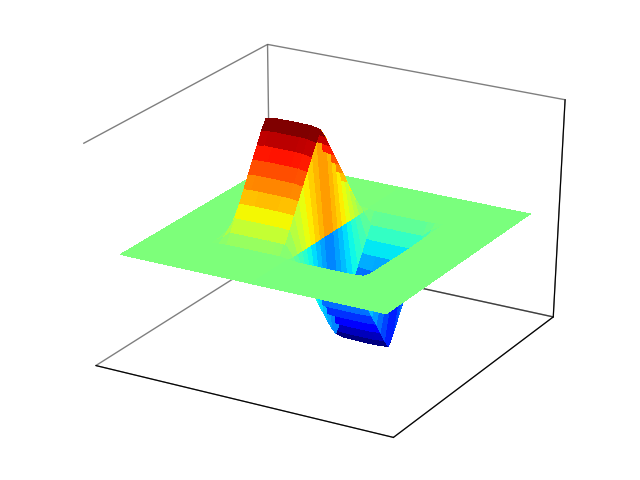
\includegraphics[width=0.35\columnwidth]{Figures/LME_17.3_Shape_Fun_dx.png}
    % \resizebox{0.54\columnwidth}{!}{%
    % \input{Figures/LME_17.3_Shape_Fun_dx.png}
    % }
    \label{fig:LME_17.3_Shape_Fun_dx}
  }
  \subfloat{
    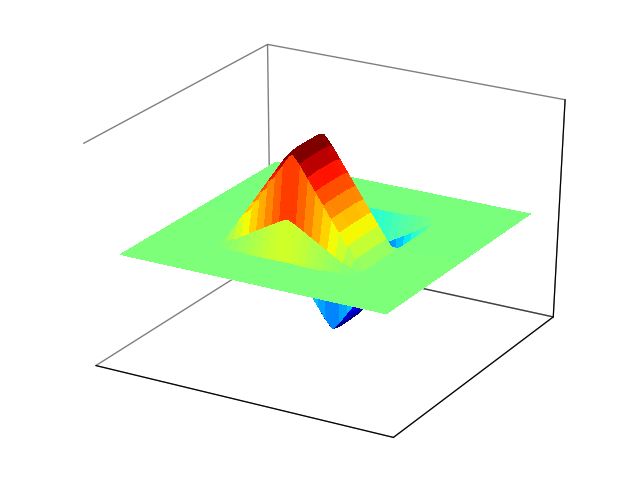
\includegraphics[width=0.35\columnwidth]{Figures/LME_17.3_Shape_Fun_dy.png}
    % \resizebox{0.54\columnwidth}{!}{%
    % \input{Figures/LME_17.3_Shape_Fun_dx.png}
    % }
    \label{fig:LME_17.3_Shape_Fun_dy}
  }
  %%%%%%%%%%%%%%%%%%%%%%%%%%%%%%%%%%%%%%%%%%%%%% 
  \qquad
  %%%%%%%%%%%%%%%%%%%%%%%%%%%%%%%%%%%%%%%%%%%%%% 
  \subfloat{
    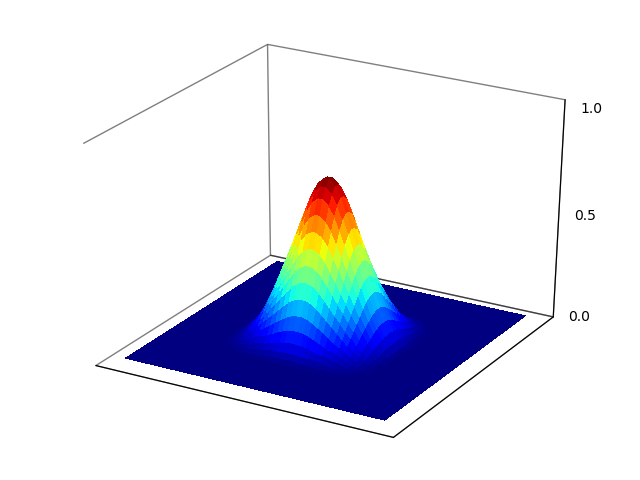
\includegraphics[width=0.35\columnwidth]{Figures/GIMP_Shape_Fun.png}
    % \resizebox{0.3\columnwidth}{!}{%
    % \input{Figures/GIMP_Shape_Fun.png}
    % }
    \label{fig:GIMP_Shape_Fun}
  }
  \subfloat{
    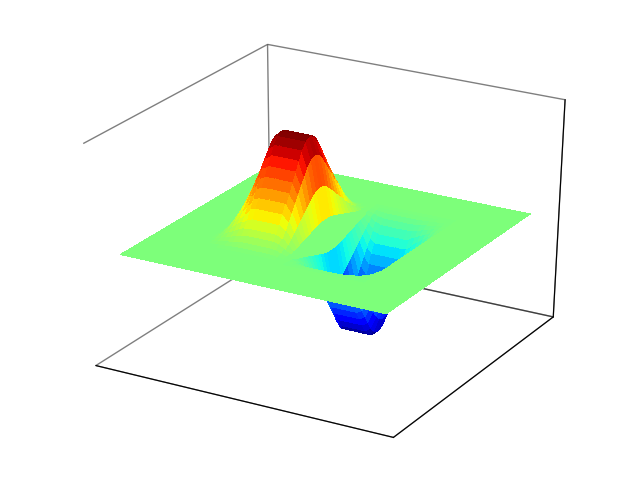
\includegraphics[width=0.35\columnwidth]{Figures/GIMP_Shape_Fun_dx.png}
    % \resizebox{0.54\columnwidth}{!}{%
    % \input{Figures/GIMP_Shape_Fun_dx.png}
    % }
    \label{fig:GIMP_Shape_Fun_dx}
  }
  \subfloat{
    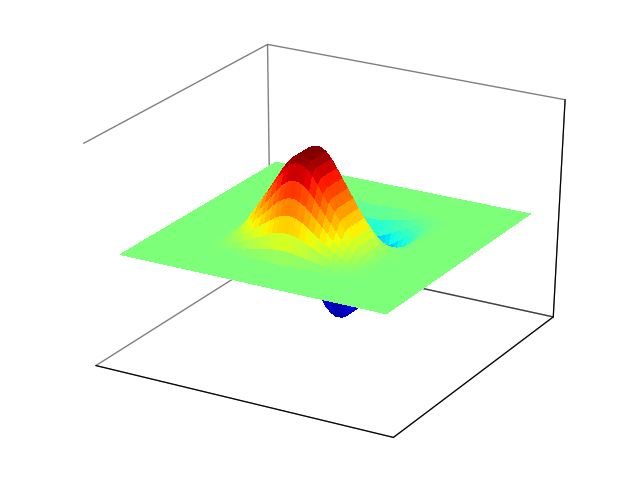
\includegraphics[width=0.35\columnwidth]{Figures/GIMP_Shape_Fun_dy.png}
    % \resizebox{0.54\columnwidth}{!}{%
    % \input{Figures/GIMP_Shape_Fun_dy.pgf}
    % }
    \label{fig:GIMP_Shape_Fun_dy}
  }
  %%%%%%%%%%%%%%%%%%%%%%%%%%%%%%%%%%%%%%%%%%%%%% 
  \qquad
  %%%%%%%%%%%%%%%%%%%%%%%%%%%%%%%%%%%%%%%%%%%%%%
  \subfloat{
    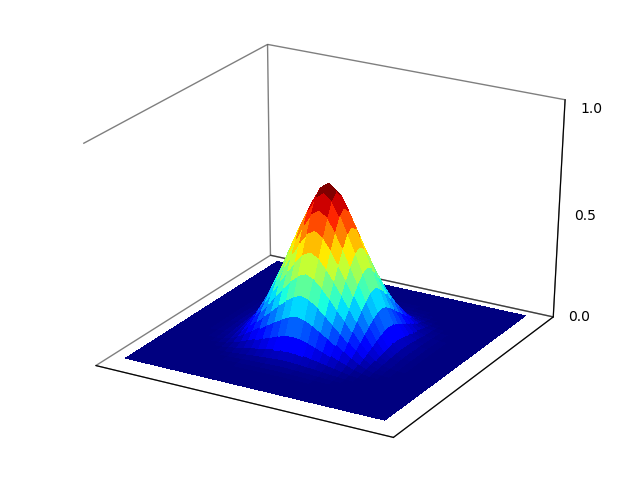
\includegraphics[width=0.35\columnwidth]{Figures/LME_10.0_Shape_Fun.png}
    % \resizebox{0.3\columnwidth}{!}{%
    % \input{Figures/LME_17.3_Shape_Fun.png}
    % }
    \label{fig:LME_10.0_Shape_Fun}
  }
  \subfloat{
    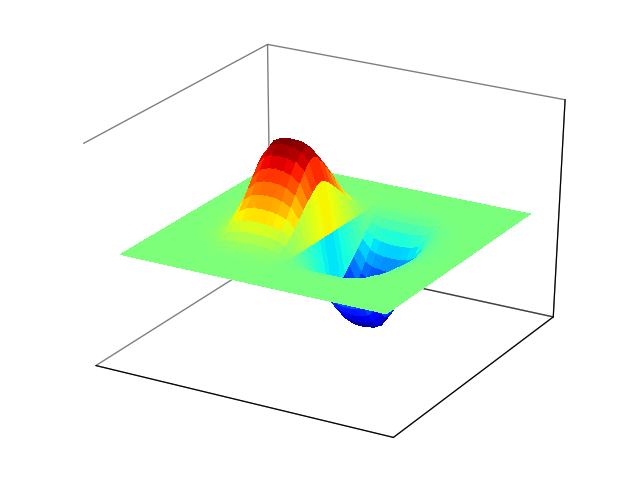
\includegraphics[width=0.35\columnwidth]{Figures/LME_10.0_Shape_Fun_dx.png}
    % \resizebox{0.54\columnwidth}{!}{%
    % \input{Figures/LME_17.3_Shape_Fun_dx.png}
    % }
    \label{fig:LME_10.0_Shape_Fun_dx}
  }
  \subfloat{
    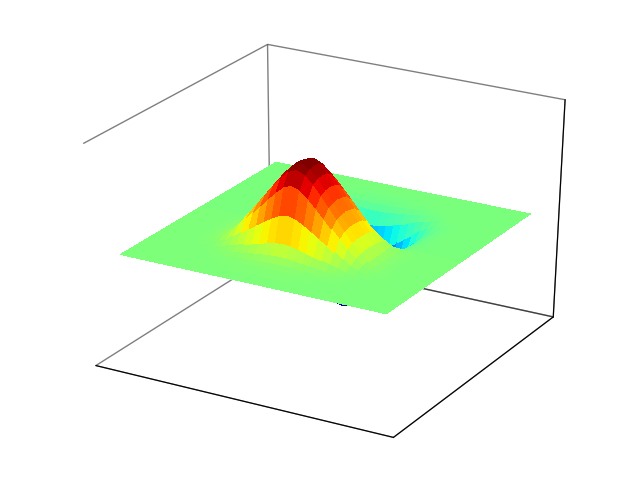
\includegraphics[width=0.35\columnwidth]{Figures/LME_10.0_Shape_Fun_dy.png}
    % \resizebox{0.54\columnwidth}{!}{%
    % \input{Figures/LME_17.3_Shape_Fun_dx.png}
    % }
    \label{fig:LME_10.0_Shape_Fun_dy}
  }
  %%%%%%%%%%%%%%%%%%%%%%%%%%%%%%%%%%%%%%%%%%%%%% 
  \qquad
  %%%%%%%%%%%%%%%%%%%%%%%%%%%%%%%%%%%%%%%%%%%%%%  
  \subfloat{
    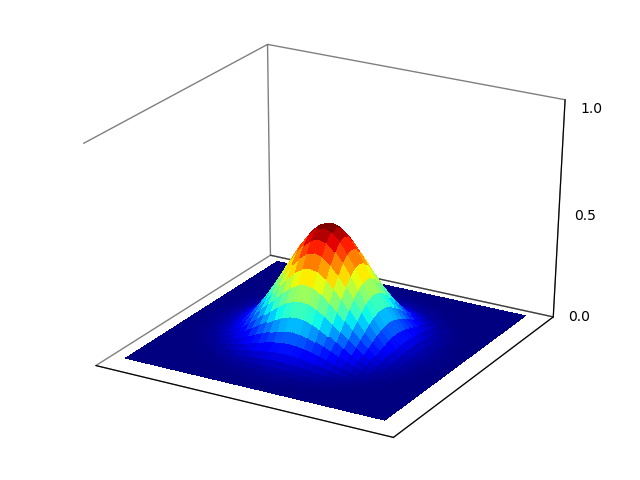
\includegraphics[width=0.35\columnwidth]{Figures/LME_7.0_Shape_Fun.png}
    % \resizebox{0.3\columnwidth}{!}{%
    % \input{Figures/LME_17.3_Shape_Fun.png}
    % }
    \label{fig:LME_7.0_Shape_Fun}
  }
  \subfloat{
    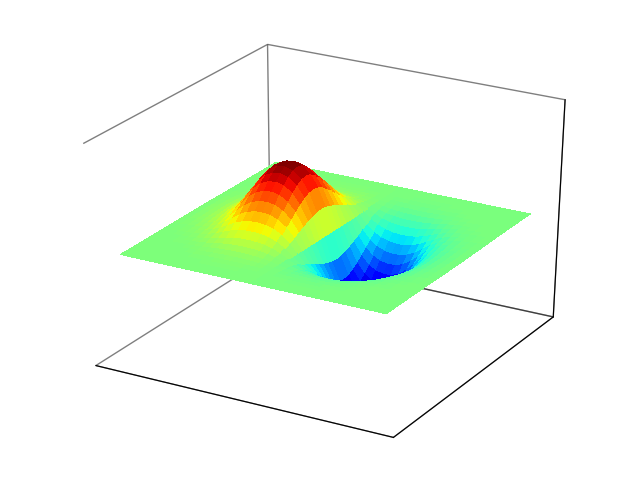
\includegraphics[width=0.35\columnwidth]{Figures/LME_7.0_Shape_Fun_dx.png}
    % \resizebox{0.54\columnwidth}{!}{%
    % \input{Figures/LME_17.3_Shape_Fun_dx.png}
    % }
    \label{fig:LME_7.0_Shape_Fun_dx}
  }
  \subfloat{
    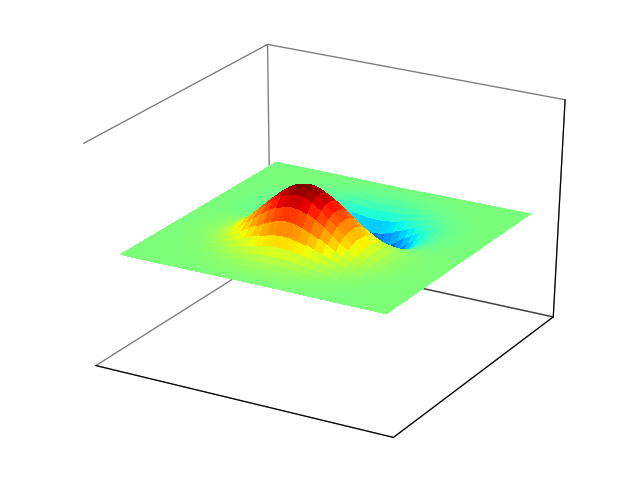
\includegraphics[width=0.35\columnwidth]{Figures/LME_7.0_Shape_Fun_dy.png}
    % \resizebox{0.54\columnwidth}{!}{%
    % \input{Figures/LME_17.3_Shape_Fun_dx.png}
    % }
    \label{fig:LME_7.0_Shape_Fun_dy}
  }
  %%%%%%%%%%%%%%%%%%%%%%%%%%%%%%%%%%%%%%%%%%%%%% 
  \qquad
  %%%%%%%%%%%%%%%%%%%%%%%%%%%%%%%%%%%%%%%%%%%%%%  
  \subfloat{
    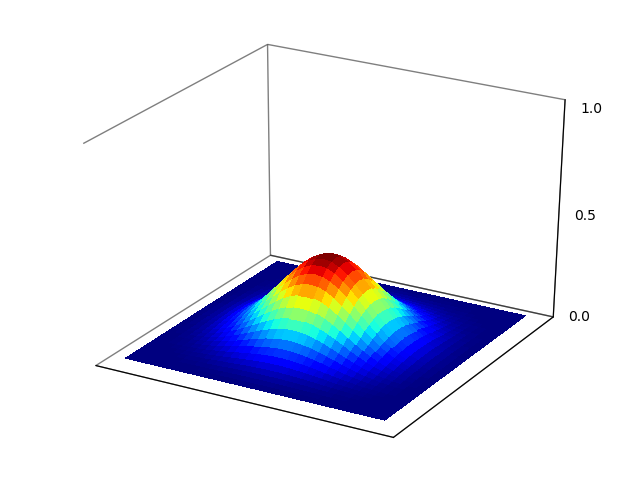
\includegraphics[width=0.35\columnwidth]{Figures/LME_5.0_Shape_Fun.png}
    % \resizebox{0.3\columnwidth}{!}{%
    % \input{Figures/LME_17.3_Shape_Fun.png}
    % }
    \label{fig:LME_5.0_Shape_Fun}
  }
  \subfloat{
    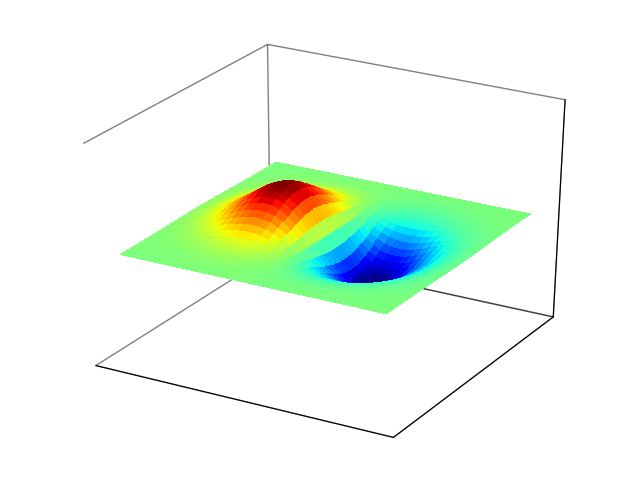
\includegraphics[width=0.35\columnwidth]{Figures/LME_5.0_Shape_Fun_dx.png}
    % \resizebox{0.54\columnwidth}{!}{%
    % \input{Figures/LME_17.3_Shape_Fun_dx.png}
    % }
    \label{fig:LME_5.0_Shape_Fun_dx}
  }
  \subfloat{
    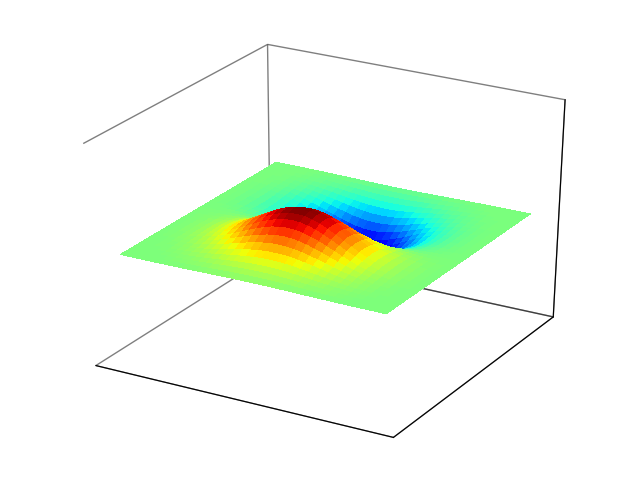
\includegraphics[width=0.35\columnwidth]{Figures/LME_5.0_Shape_Fun_dy.png}
    % \resizebox{0.54\columnwidth}{!}{%
    % \input{Figures/LME_17.3_Shape_Fun_dx.png}
    % }
    \label{fig:LME_5.0_Shape_Fun_dy}
  }
  \caption{Local max-ent shape functions for a two-dimensional
    arrangement of nodes, and spatial derivatives for several values
    of $\gamma = \beta/h^2$.}
  \label{fig:LME_MPM}
\end{figure}

\section{Numerical results : 1D Elastic bar}
\label{sec:dynamic-benchmark}

In this section, the benchmark proposed by Dyka \& Ingel
(1995)\cite{Dyka1995} is considered to illustrate the
capacity of MPM \cite{Sulsky1994} and OTM
models to avoid tensile instabilities. 

In the one-dimensional bar sketched in
the figure \ref{fig:Dyka_Bar}, the left end of the bar is fixed and
the right and an initial velocity $v_0 = 5\ m/s$ is given to the last
quarter of it in the x positive direction. The length of it is 0.1333
meters with an unit section. The elastic parameters consider for this
test are:
\begin{itemize} 
\item  Density : $7833\ kg/m3$
\item  Poisson ratio : $0$
\item  Elastic modulus : $200 \cdot 10^9\ Pa$
\end{itemize}

The results are provided for the explicit predictor-corrector version of the
MPM scheme (Algorithm \ref{alg:PCE-algorithm}) and OTM algorithms. For MPM, piecewise-
linear, uGIMP and \textit{max-ent} basis functions are employed. The OTM
algorithm is used only with \textit{max-ent} shape functions. 

\begin{figure}\sidecaption
  \centering
  \resizebox{0.8\hsize}{!}{
    \begin{tikzpicture} 
  \scaling{2}; 
  % Nodos 
  \point{a}{0}{1};
  \point{b}{3.75}{1};
  \point{c}{5}{1};
  % Barras
  \beam{2}{a}{b};
  \beam{2}{b}{c};
  % Apoyos
  \support{3}{a}[270];
  % Fuerzas
  \lineload{4}{b}{c}[1][0.2];
  \notation{5}{b}{c}[$5\ m/s$][.5][below][2];
  % Nombres de nodos
  \notation{1}{a}{A}[below right];
  \notation{1}{b}{B}[below right];
  \notation{1}{c}{C}[below right];
  % Cotas
  \dimensioning{1}{a}{b}{0.5}[{\unit[3/4]{L}}];
  \dimensioning{1}{b}{c}{0.5}[{\unit[1/4]{L}}];
\end{tikzpicture}
}
  \caption{Geometrical description of the Dyka \cite{Dyka1995} bar. }
  \label{fig:Dyka_Bar}
\end{figure}

The boundary conditions are:
\begin{equation}
  \label{eq:3}
  \sigma \rvert_{x=L} = 0 \quad , \quad v \rvert_{x=0} = 0
\end{equation}

The analytical solution in terms of velocity
\ref{fig:vel_analytics_dyka}, and stress
\ref{fig:stress_analytics_dyka} can be found in the appendix
\ref{app:analytical_sol} given by the Method of characteristics. For
the convergence analysis, the root-mean-square (RMS) error in the
displacement is computed. RMS error is defined as follows

\begin{equation}
  \label{eq:RMS}
  RMS = \sqrt{\frac{1}{N} \sum^{N}_p \left( \phi_p - \hat{\phi}_p \right)}
\end{equation}

\subsection{Error analysis MPM vs uGIMP vs MPM-\textit{max-ent}}
\label{sec:study-error}



\subsection{MPM versus OTM}
\label{sec:mpm-versus-otm}


\section{Conclusions}
\label{sec:conclusions}

Building upon the idea of anisotropic shape functions
\cite{Arroyo2006}, \cite{Kochmann2019} introduced an enhanced version of the
original local max-ent scheme, which uses an anisotropic support to
deal with tensile inestability.


%\begin{acknowledgements}
%If you'd like to thank anyone, place your comments here
%and remove the percent signs.
%\end{acknowledgements}

% Authors must disclose all relationships or interests that 
% could have direct or potential influence or impart bias on 
% the work: 
%
\section*{Conflict of interest}
%
The authors declare that they have no conflict of interest.


\appendix
\section{The analytical solution of the 1D Dyka benchmark}
\label{app:analytical_sol}

For the derivation of this analytical solution we will consider  the
dynamic behaviour of a 1D elastic bar. The governing equations are the
following: (i) The balance of linear momentum,
\begin{equation}
  \label{eq:1D-balance-linear-momentum}
  \rho\ \Deriv{v}{t} = \Deriv{\sigma}{x} + \rho\ b,
\end{equation}
where $\sigma$ is the stress value, $\rho$ is the density,
$v$ is the velocity, and $b$ are the body
forces. (ii) The constitutive model, which for convenience of the
following developments will be written in terms of displacement and
velocities as, 
\begin{equation}
  \label{eq:1D-constitutive-equation}
  \Deriv{\sigma}{t} = E \Deriv{\varepsilon}{t},
\end{equation}
where $E$ is the elastic modulus. (iii) The compatibility equation
also in terms of the velocity field,
\begin{equation}
  \label{eq:CompatibilityEquation_e}
  \Deriv{\varepsilon}{t} = \Deriv{v}{x}.
\end{equation}
Next for simplicity, we remove the body forces from
\eqref{eq:1D-balance-linear-momentum}, and we will introduce
\eqref{eq:CompatibilityEquation_e} in
\eqref{eq:1D-constitutive-equation}, so we get the following system of equations,
\begin{align}
  \label{eq:1D-balance-linear-momentum-II}
  \Deriv{v}{t} &= \frac{1}{\rho}\ \Deriv{\sigma}{x}, \\
  \label{eq:1D-constitutive-equation-II}
  \Deriv{\sigma}{t} &= E\ \Deriv{v}{x}.
\end{align}

Introducing \eqref{eq:1D-constitutive-equation-II} in
\eqref{eq:1D-balance-linear-momentum-II} and expressing the remaining
equation in terms of the displacement, we reach the 1D wave
equation for linear elastic materials,
\begin{equation}
  \label{eq:1D-wave-elastic}
  \Deriv[2]{u}{t} = \frac{E}{\rho}\ \Deriv[2]{u}{x} = c^2\ \Deriv[2]{u}{x}
\end{equation}
where we have introduced the wave celerity $c$ as,
\begin{equation}
  \label{eq:1D-elastic-wave-celerity}
  c = \sqrt{\frac{E}{\rho}}
\end{equation}
Alternative, rearranging both equations
\eqref{eq:1D-balance-linear-momentum-II} and
\eqref{eq:1D-constitutive-equation-II} it is possible to join them in a
single system of equations as,
\begin{equation}
  \label{eq:System-stress-velocity}
  \Deriv{}{t} \left[
    \begin{array}{c}
      \sigma \\
      v
    \end{array}
  \right] + \left[
    \begin{array}{cc}
      0 & - E \\
      - 1/\rho & 0 
    \end{array} \right] \left[
    \begin{array}{c}
      \Deriv{\sigma}{x} \\
      \Deriv{v}{x}
    \end{array}
  \right] = \Vector{0}.
\end{equation}
This expression can be written in a more compact format as,
\begin{equation}
  \label{eq:System-stress-velocity-II}
  \Deriv{\Vector{\phi}}{t} + \Matrix{A}\Deriv{\Vector{\phi}}{x} = \Vector{0}
\end{equation}
where both variables are joined in a single vectorial variable
$\Vector{\phi}$ and $\Matrix{A}$ in coupling matrix between both equations,
\begin{equation*}
  \Vector{\phi} = \left[
    \begin{array}{c}
      \sigma \\
      v
    \end{array}
  \right],\quad 
  \Matrix{A} =  \left[
    \begin{array}{cc}
      0 & - E\\
      - 1/\rho & 0 
    \end{array} \right].
\end{equation*}
Note that the nature of \label{eq:eq:System-stress-velocity-II} is still
hyperbolic despite the fact it does not have a second order
temporal derivative as \eqref{eq:1D-wave-elastic}. A proof of this can
be easily obtained if we get the zeros of the hypersurface defined by
\eqref{eq:1D-wave-elastic}. And later the eigenvalues of $\Matrix{A}$
in \eqref{eq:System-stress-velocity-II}. In both cases, eigenvalues
are real and distinct ($\lambda = \pm \sqrt{\frac{E}{\rho}}$),
therefore the system is called strictly hyperbolic.

For a more general description in the following, we will assume that $\Matrix{A}$ has $n$
different eigenvalues $\{ \lambda_1, \lambda_2, \ldots, \lambda_i, \ldots
\lambda_n \}$ and $n$ eigenvectors $\{ \vec{x}^1, \vec{x}^2, \ldots,
\vec{x}^i, \ldots \vec{x}^n \}$ satisfying that $\tens{A} \vec{x} =
\lambda \vec{x} $. Now we introduce the matrix $\Matrix{P}$ whose columns are the $n$
eigenvalues $\Vector{x}$
\begin{equation}
  \label{eq:P-matrix}
\Matrix{P} = \{ \vec{x}^1, \vec{x}^2, \vec{x}^3, \ldots \vec{x}^n \}.
\end{equation}
Diagonalizing $\Matrix{A}$ using $\Matrix{P}$ we get
\begin{equation}
  \label{eq:Lambda-matrix}
  \Lambda = \Matrix{P}^{-1} \Matrix{A}\ \Matrix{P},
\end{equation}
where $ \Lambda_{ii} = \lambda_i$. Next we will define a vector $\Vector{\Re}$ such that:
\begin{equation}
  \label{eq:Riemann-definition}
  \Vector{\phi} = \Matrix{P}\ \Vector{\Re}
\end{equation}
we will assume to be integrable. Expanding the above expression with
the chain rule and passing the matrix $\Matrix{P}$ to left hand side
of the equality we get,
\begin{equation}
  \label{eq:Riemann-II}
  d \vec{\Vector{\Re}} = \Deriv{\Vector{\Re}}{t}dt + \Deriv{\Vector{\Re}}{x}dx =
  \tens{P}^{-1}\left(\Deriv{\phi}{t}dt + \Deriv{\phi}{x}dx \right)
\end{equation}
and setting the terms we get,
\begin{equation}
  \label{eq:Riemann-III}
  \Deriv{\Vector{\Re}}{t} = \Matrix{P}^{-1}\Deriv{\Vector{\phi}}{t},\quad 
  \Deriv{\Vector{\Re}}{x} = \Matrix{P}^{-1}\Deriv{\Vector{\phi}}{x}
\end{equation}
Next, if we multiply \eqref{eq:System-stress-velocity-II} by
$\Matrix{P}^{-1}$ we get:
\begin{equation}
  \label{eq:System-stress-velocity-III}
  \Matrix{P}^{-1}\Deriv{\Vector{\phi}}{t} + \left(\Matrix{P}^{-1}\Matrix{A}\Matrix{P}
  \right)\Matrix{P}^{-1} \Deriv{\Vector{\phi}}{x} = \Vector{0}
\end{equation}
finally introducing the expressions \eqref{eq:Riemann-III} we reach to
\begin{equation}
  \label{eq:System-stress-velocity-IV}
  \Deriv{\Vector{\Re}}{t} + \Lambda \Deriv{\Vector{\Re}}{x} = \Vector{0}  
\end{equation}
which consists of $n$ uncoupled equations as $\Lambda$ is
diagonal matrix as we can see in \eqref{eq:Lambda-matrix}. Each of this
equations are 1D scalar convective transport equations, with solutions
of the form:
\begin{equation}
  \label{eq:SystemEquations_sigma_v_VI}
  \Re^{(i)} = F^{(i)} \left(x - \lambda^{(i)} t \right)
\end{equation}

This uncoupled system, has, therefore, a set of $n$ characteristics.
These magnitudes $\Re_i$ which propagate along characteristics are
known as ``Riemann invariants'' of the problem. Here we have a 1D
configuration, so the domain is $\Omega : \left(0, L\right) x \left(0,
  T\right)$. For the closure of the problem we require:
\begin{itemize}
\item ``n'' initial conditions of the form $\Re_i (x,t=0) = h_i(x)$,
  where $i = {0, \ldots, n}$, and $h_i(x)$ is a vectorial function
  given by the physical variables of the problem.
\item ``n'' boundary conditions.
\end{itemize}

Now particularizing the previous equations for the 1D elastic bar
described in \cite{Dyka1995}, we get that the matrix $\Matrix{P}$
is the following:
\begin{equation*}
    \Matrix{P} =  \left[
    \begin{array}{cc}
      -\sqrt{E\rho} & \sqrt{E\rho}\\
       1 & 1 
    \end{array} \right]
\end{equation*}
and its inverse is:
\begin{equation*}
    \Matrix{P}^{-1} = \frac{1}{2} \left[
    \begin{array}{cc}
      -\frac{1}{\sqrt{E\rho}} & 1\\
      \frac{1}{\sqrt{E\rho}} & 1 
    \end{array} \right]
\end{equation*}

And introducing the value of the inverse matrix $\Matrix{P}^1$ in the
Riemann definition \eqref{eq:Riemann-definition} we get the following
system of equations,
\begin{align}
  \label{eq:Riemann-I-1D-elastic-bar}
  &\Re^{I} = \frac{1}{2\sqrt{\rho E}}\left(-\sigma + v\ \sqrt{\rho E}
    \right)\\
  \label{eq:Riemann-II-1D-elastic-bar}
  &\Re^{II} = \frac{1}{2\sqrt{\rho E}}\left(\sigma + v\ \sqrt{\rho E} \right)
\end{align}

From \eqref{eq:Riemann-I-1D-elastic-bar} and
\eqref{eq:Riemann-II-1D-elastic-bar} we can obtain the values of the
stress and the velocity as:
\begin{equation}
  \label{eq:Riemann-stress-velocity}
  v = \Re^{I} + \Re^{II} \quad , \quad \sigma = \sqrt{E \rho}\left(\Re^{II} - \Re^{I} \right)
\end{equation}

The boundary conditions are in both cases of radiation as there is not
wave in-going from the exterior. So for the left side (fixed
boundary) we get the following conditions:
\begin{equation*}
  &\Re^{I} = 0 \quad and \quad v_{x=0} = 0
\end{equation*}
Therefore $\sigma_{x=0} = \sqrt{\rho E}\Re^{II}$. And in the left side
(free boundary) we get the following conditions:
\begin{equation*}
  &\Re^{II} = 0 \quad and \quad \sigma_{x=L} = 0
\end{equation*}
Therefore $v_{x=L} = \Re^{I}$. Finally, applying this conditions in
the elastic bar sketched in \ref{fig:Dyka_Bar}, is possible to obtain
the velocity history in the right side of the bar
\ref{fig:vel_analytics_dyka} and the stress in the last quarter side of the Dyka
bar \ref{fig:stress_analytics_dyka} as is demanded in \cite{Dyka1995}.

\begin{figure}\sidecaption
  \centering
  \resizebox{\hsize}{!}{
    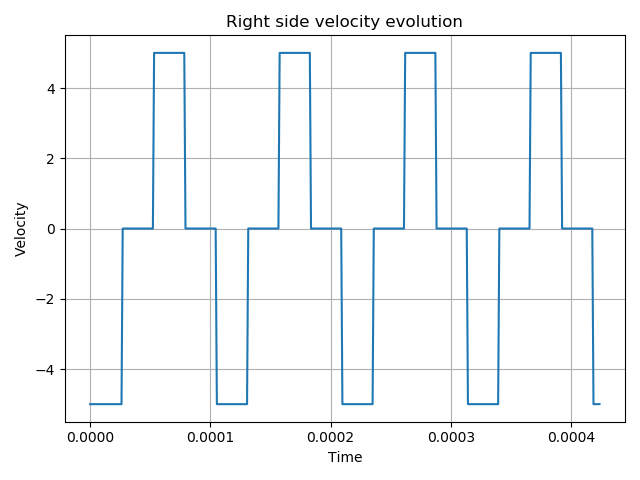
\includegraphics[width=\columnwidth]{Figures/1D_right_Velocity.png}
  }
  \caption[Velocities values in the right side of the Dyka
  bar]{Analytical solution for the velocity in the right side of the Dyka bar.}
  \label{fig:vel_analytics_dyka}
\end{figure}

\begin{figure}\sidecaption
  \centering
  \resizebox{\hsize}{!}{
    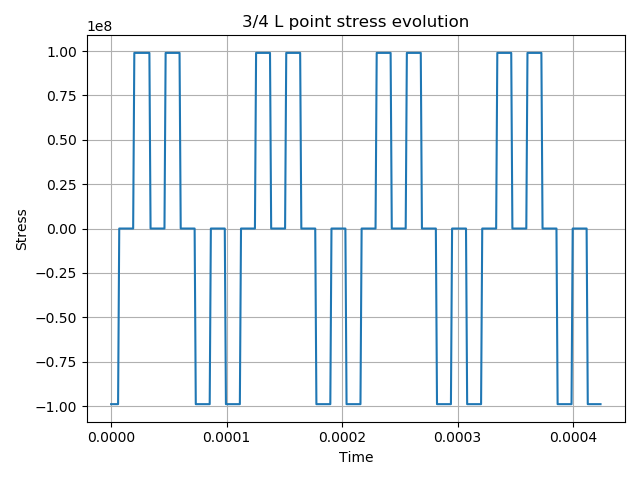
\includegraphics[width=\columnwidth]{Figures/1D_left_Stress.png}
  }
  \caption[Stress values in the last quarter side of the Dyka
  bar]{Analytical solution for the stress in the last quarter of the Dyka bar.}
  \label{fig:stress_analytics_dyka}
\end{figure}



% BibTeX users please use one of
%\bibliographystyle{spbasic}      % basic style, author-year citations
\bibliographystyle{spmpsci}      % mathematics and physical sciences
%\bibliographystyle{spphys}       % APS-like style for physics
\bibliography{Biblio.bib}   % name your BibTeX data base

\end{document}
% end of file template.tex


%%% Local Variables:
%%% mode: latex
%%% TeX-master: t
%%% End:

